\documentclass[thesis]{subfiles}

\begin{document}

\OnlyInSubfile{\setcounter{chapter}{2}}
\chapter{Molecular simulations}
\label{sec:molsim}

Macroscopic modeling methods such as the ones I discussed in the previous
chapter are not always sufficiently precise to gain a complete understanding of
the phenomenon at play. In particular, as these methods describe the systems at
the macroscopic level, they don't take into account the individual atoms, and
the interactions between them: they don't describe the \emph{chemistry} of the
system. Statistical thermodynamics is a tool that we can use to bring together
the microscopic description of matter and the macroscopic behavior and
characteristics of the system (pressure, temperature, \dots).

In this chapter, I will derive and recall some concepts from statistical
thermodynamics I used during my PhD. For a more in-depth description of
statistical mechanics, I recommend the book of Tuckerman\cite{Tuckerman2010}. I
will then present the molecular simulation methods used to sample thermodynamic
ensembles in practice. On this section, I recommend the book of Frenkel and
Smit\cite{Frenkel2002}.

\section{Statistical thermodynamics}
\label{sec:statistical-thermo}

\subsection{Maxwell-Boltzmann statistics}

We will consider a molecular system containing $N$ individual atoms behaving as
classical particles with individual positions $\r_i$, identical masses $m$ and
momentum $\p_i$. Supposing that these particles are in some container of fixed
volume $V$, and at thermal equilibrium with a thermostat at temperature $T$,
they evolve in the canonical or $NVT$ ensemble. Finally, we will also assume
that the atoms in the system follow the Maxwell-Boltzmann statistics, \ie that
the probability density of finding the system in a state of internal energy
$E_i$ is given by:
\[\mathcal{P}_i = \frac{1}{N!\ h^{3N}\ Z} e^{-\beta\, E_i}, \label{eq:maxwell-boltzmann}\]
where $\beta = 1 / k_B T$ with $k_B$ the Boltzmann constant and $N!\ h^{3N}\ Z$
is a normalization constant. To be more precise, particles would either follow
Bose--Einstein statistics for bosons (particles with a full integer spin, such as
photons) or the Fermi–Dirac statistics for fermions (particles with half-integer
spin, such as electrons or protons). But as both Bose-Einstein and Fermi-Dirac
statistics reduce to the Maxwell-Boltzmann distribution when the temperature is high
enough, we will use this distribution instead.

We define the state of a system by the values taken by all the positions $\r_i$
and all the momentum $\p_i$ of all the $N$ atoms in the system. The state of the
system is then defined by $6N$ variables, or a point in a vector space of $6N$
dimensions called the \emph{phase space}. In order to compute the energy of a
state, we will describe the interactions between the atoms by a potential energy
$U(\r^N)$, with no explicit dependency on time. Then, we can compute the total
energy of a state using the classical Hamiltonian of the system:
\[H(\r^N, \p^N) = \sum_i^N \frac{\p_i^2}{2 m} + U(\r^N);\]
where I use $\r^N$ and $\p^N$ as shorthand for the set of all positions
$\{\r_i\}$ and momentum $\{\p_i\}$ respectively.

The last element in equation~\eqref{eq:maxwell-boltzmann} we need to compute is
the so-called \emph{partition function} $Z$. We note that the probability for
the system to be anywhere in the phase space $\Phi$ should be 1, which gives us:
\[\iint_\Phi \mathcal{P}_i \; \d\r^N \d\p^N = 1.\]
And finally:
\[Z = \frac{1}{N!\ h^{3N}} \iint_\Phi e^{-\beta\, H(\r^N, \p^N)} \ \d\r^N \d\p^N\]
where the Planck constant $h$ is used as a normalization factor used to make
sure that $Z$ has the right dimension, and the $N!$ factor comes from the fact
that particles are not distinguishable one from another.

We can already compute at least a part of this integral by separating the
kinetic and potential energy terms in the Hamiltonian:
\[Z = \frac{1}{N!\ h^{3N}} \left(\prod_i^{3N} \int e^{-\beta\, \p_i^2 / 2 m} \ \d \p_i \right) \left(\iiint_V e^{-\beta\, U(\r^N)} \ \d\r^N \right) \]
where the potential energy integral is over all the accessible volume. The
kinetic energy term is a product of Gaussian integrals, and gives us the
following expression for the partition function:
\[Z = \frac{1}{N!} \prod_i^{3N} \sqrt{\frac{2\pi m}{\beta h^2}} \iiint_V e^{-\beta\, U(\r^N)} \ \d\r^N\]
$\lambda = \sqrt{\beta h^2 / 2\pi m}$ is the de Broglie thermal wavelength for a
particle with mass $m$, and is homogeneous to a distance. This gives the final
expression for the partition function:
\[Z = \frac{1}{N!\ \lambda^{3N}} \iiint_V e^{-\beta\, U(\r^N)} \ \d\r^N \label{eq:partition-function}\]
And the corresponding probability for the system to be in a given conformation
without constrains on the kinetic energy:
\[\mathcal{P}_i = \frac{1}{N!\ \lambda^{3N}\ Z}\ e^{-\beta\, U(\r^N)}\]

\subsubsection{Thermodynamic quantities from the partition function}

It is possible to use the knowledge of the partition function to compute some
of the macroscopic properties of our system. For examples, the internal energy
is the average value of the Hamiltonian:
\[ \mathcal{U} = \frac{1}{Z} \iiint_\Phi H \ e^{-\beta\, H} \]
If we express $H e^{-\beta\, H}$ as the partial derivative of $e^{-\beta\, H}$ with
respect to $\beta$ we get
\[\mathcal{U} = - \frac{1}{Z} \frac{\partial}{\partial \beta} \iiint_\Phi e^{-\beta\, H} \]
\[\mathcal{U} = - \frac{1}{Z} \frac{\partial Z}{\partial \beta}\]

The entropy of a system can be computed from the probability density
$\mathcal{P}$, using the relation:
\[S = -k_B \iint_\Phi \mathcal{P} \ln \mathcal{P}, \]
which reduces after some calculations to
\[S = k_B \left[\ln Z - \frac{\beta}{Z} \frac{\partial Z}{\partial \beta} \right].\]
The free energy definition $F = \mathcal{U} - TS$ the gives us:
\[F = - \frac 1 \beta \ln Z\]

Knowing the free energy, we can use all the results from classical
thermodynamics to compute some other properties of the system:
\[P = - \frac{\partial F}{\partial V} \qquad \qquad \mu = - \frac{\partial F}{\partial n}\]

\newpage
\subsubsection{Observables}

The probability for the system to be in a given state gives us the missing link
between microscopic and macroscopic properties of the system. We can express a
macroscopic observable property $A$ that we can also compute or measure at a
microscopic level using Maxwell-Boltzmann statistics:
\[A = \braket{A} = \iiint_\Phi \mathcal{P}_i \ A_i.\]
The value of $A$ at a macroscopic level is the same value as the ensemble
average $\braket{A}$, which depends on both the value of the property in a given
macroscopic state $A_i$, and the probability of the system to be in this state.
Using equations~\eqref{eq:maxwell-boltzmann} and~\eqref{eq:partition-function}
together, we can express the average value for any observable property in the
canonical ensemble:
\[\braket{A} = \frac{\iiint_\Phi \d\r^N \d\p^N \; A(\r^N, \p^N) \ e^{-\beta\, H(\r^N, \p^N)}}{\iiint_\Phi \d\r^N \d\p^N \; e^{-\beta\, H(\r^N, \p^N)}}. \label{eq:observable}\]

\subsubsection{Sampling}

This theoretical approach to define macroscopic properties from microscopic data
is useless unless we can compute the integrals over the whole phase space $\Phi$
in~\eqref{eq:observable}. But computing this integral explicitly in all but the
simplest cases will prove difficult, as the phase space is a $6N$ dimensional
vector space, and values for $N$ range from a few hundred all the way up to
Avogadro number. But in general, a lot of states in the phase space are not
relevant when computing the integral, mainly because their energy is too high
and their probability becomes negligible. So instead of computing the whole
integral, we resort to only using a finite number of samples in the phase space,
which we try to pick as the most relevant. In a semi-formal manner, we try to
generate a set of points $\phi$ inside the phase space, such that
\[\braket{A} \approx \frac{\sum_\phi A(\r^N, \p^N) e^{-\beta\, H(\r^N, \p^N)}}{\sum_\phi e^{-\beta\, H(\r^N, \p^N)}}.\]

This is the underlying idea of molecular simulation, \ie the numerical sampling
of phase space based on the knowledge of a way to calculate the energy of each
state. There are a few algorithms we can use to do this sampling and generate
the set $\phi$ of points we will use to compute a given property. I will discuss
two of them below: the Metropolis Monte Carlo (MC) method, and Molecular
Dynamics (MD). If we can get these algorithms to generate a set of states in
the phase space according to the Maxwell-Boltzmann probability, with the same
state appearing possibly more than once in the set, we can simplify the
calculation of ensemble average of observables even further. For a set of $m$
physically representative states indexed by $\alpha$, the average reads as:
\[\braket{A} \approx \frac 1 m \sum_\alpha^m A(\r_\alpha^N, \p_\alpha^N). \label{eq:observable:r-only}\]

\newpage
\subsection{Thermodynamic ensembles}

Until now, all the calculations were done in the canonical or $NVT$ ensemble,
following the Maxwell-Boltzmann distribution. It is possible to show that in
other thermodynamic ensembles one can write a similar probability distribution
for the phase space. The partition function defined by the normalization of
these probability distributions can be used to compute all of the properties of
the system, and in particular the associated thermodynamic potential.

\subsubsection{Isothermal-isobaric ensemble} In the $NPT$ ensemble, the volume
$V$ is a free variable, and the probability for the system to be in a given
configuration is:
\[ \mathcal{P}_{NPT} = \frac{1}{N!\ \lambda^{3N}\ \Delta} \kern1em e^{-\beta \left[U(\r^N) \ + \ PV\right]} \]
\[ \Delta = \frac{1}{N!\ \lambda^{3N}} \int \d V \iiint_V \d\r^N \; e^{-\beta \left[U(\r^N) \ + \ PV\right]} \]

And the free energy is given by:
\[G = - \frac 1 \beta \ln \Delta.\]

\subsubsection{Grand canonical ensemble}

In the $\mu VT$ ensemble, the number of atoms $n_i$ can vary while the
associated chemical potential $\mu_i$ is fixed. The probability for the system
to be in a state is given by:
\[ \mathcal{P}_{\mu VT} = \frac{1}{N!\ \lambda^{3N}\ \Theta} \kern1em e^{-\beta \left[U(\r^N) \ - \ \sum_i \mu_i n_i \right]} \label{eq:uVT-probability} \]
\[ \Theta = \kern-2.5em \sum_{\substack{N=0 \\[0.5ex] \kern2.75em N=n_1+n_2+\dots}}^\infty \kern-2em \frac{1}{N!\ \lambda^{3N}} \iiint_V \d\r^N \d\p^N \; e^{-\beta \left[U(\r^N) \ - \ \sum_i \mu_i n_i \right]} \]

\subsubsection{Osmotic ensemble}

In the osmotic ($N_\text{host} \ \mu \ PT$) ensemble, the number of atoms $n_i$
of guest molecules and the volume $V$ can vary while the associated chemical
potential and pressure are constants. The probability for the system to be in a
state is given by:
\[ \mathcal{P}_{\mu VT} = \frac{1}{N!\ \lambda^{3N}\ \zeta} \kern1em e^{-\beta \left[H(\r^N, \p^N) \ + \ PV \ - \ \sum_i \mu_i n_i \right]} \label{eq:probably:uvt}\]
\[ \zeta = \kern-2.5em \sum_{\substack{\kern1.2em N=N_\text{host} \\[0.5ex] \kern2.6em N=n_1+n_2+\dots}}^\infty \kern-1em \frac{1}{N!\ \lambda^{3N}} \int \d V \iiint_V \d\r^N \d\p^N \; e^{-\beta \left[U(\r^N) \ + \ PV \ - \ \sum_i \mu_i n_i \right]} \]
Here, $N$ is the total number of atoms in the system, counting both the fixed
host atoms and the varying atoms of the guest. The $\sum_i \mu_i n_i$ sum only
run on the guest species.

\newpage
\section{Computing energy of a molecular system}

Before we can compute properties of a system using
equation~\eqref{eq:observable:r-only}, we need to be able to compute the energy
$U(\r^N)$ associated with any configuration of the system. I will describe the
two main approaches used to do so in this section.

\subsection{Quantum calculations}

The most generic way to compute the energy of a configuration of a system is to
solve the Schrödinger equation for the $N$ electrons in the system evolving in
the potential created by the $M$ nuclei; given here in atomic units:
\[\left[-\frac 1 2 \sum_i^N \nabla^2_i - \sum_i^N \sum_j^M \frac{Z_j}{|\r_i - \r_j|} + \sum_i^N \sum_{j>i}^N \frac{1}{|\r_i - \r_j|} \right] \psi(r) = E \psi(r)\]
There is no analytic solution for this equation, and the high dimensionality of
the solution space ($\approx 3 N$) make numeric resolution very difficult.
Instead, we use approximated methods to solve the equation, such as Quantum
Monte Carlo, Hartree-Fock and post Hartree-Fock methods, or the Density
Functional Theory (DFT). Of these methods I will only present DFT, as it is the
most widely used today, and particularly suitable for the study of systems with
hundreds of atoms and periodic boundary conditions. The central idea of DFT is
to solve these equations in terms of the total electronic density $n(\r)$, and
then write the total energy of the system as a functional of the density $E[n]$.
I will explain in more details in section~\ref{sec:dft} how DFT relates to the
Schrödinger equation, and how minimizing the energy functional gives us the
energy of the system in the ground state.

Even when using DFT, solving the Schrödinger equation is costly in term of
computing time, and imposes a limit on both the time and length scale of systems
we can study. As of 2019, using standard high performance computing cluster, we
can use DFT to study systems containing up to 1000 atoms on a time scale of up
to \SI{100}{ps}. While these numbers increased a lot in recent years due to
improvements in software used for DFT and in computing hardware, they are still
many systems of interest that we cannot study with DFT. If the electronic
density does not vary much across the subspace of phase space we are interested
in --- \ie no bond creation or breakage; no charge transfer --- then using
classical potentials or force fields can be a good approximation of the real
energy.

\subsection{Classical force fields}
\label{sec:classical-ff}

A force field is an educated guess on the functional form of the energy of a
system, decomposed as a sum of simple terms with physical meanings. It is a
classical and empirical approximation of the real, quantum potential energy
surface. The usual decomposition is the following:
\[V(\r) = \sum_i \sum_j V_\text{pairs}^{ij} + \sum_\alpha V_\text{molecular}^\alpha + V_\text{coulomb} \]
where $V_\text{coulomb}$ is the Coulombic interaction between charged atoms,
$V_\text{molecular}$ represent the internal molecular energy and
$V_\text{pairs}$ represent the non-bonded pairs interactions. These terms are
often broken down even further. For example, the simplest form possible for
$V_\text{coulomb}$ is to use fixed point charges attributed to each atom during
the force field parametrization. If this is not enough to reproduce the
properties of the system of interest, we can use diffuse Gaussian charges
instead, or add a term describing atomic polarization. $V_\text{pairs}$ is used
to reproduce both the dispersion interactions and the Pauli repulsion between
atoms at short distances. $V_\text{molecular}$ represent the intra-molecular
interactions, and is usually decomposed over bonded coefficients:
\[V_\text{molecular} = \sum_\text{bonds} V_\text{bond}(r) + \sum_\text{angles} V_\text{angle}(\theta) + \sum_\text{dihedrals} V_\text{dihedral}(\phi)\]
Each energy term only depends on the type of bonded atoms, and a single scalar
variable: the distance $r$ between the two atoms for bonds contributions; the
3-body angle $\theta$ for angles contributions, and the 4-body dihedral angle
$\phi$ or out of plane distance $d$ for dihedral angles contributions. These
variables are illustrated in figure~\ref{fig:force-fields:molecular}.

\begin{figure}[ht]
    \centering
    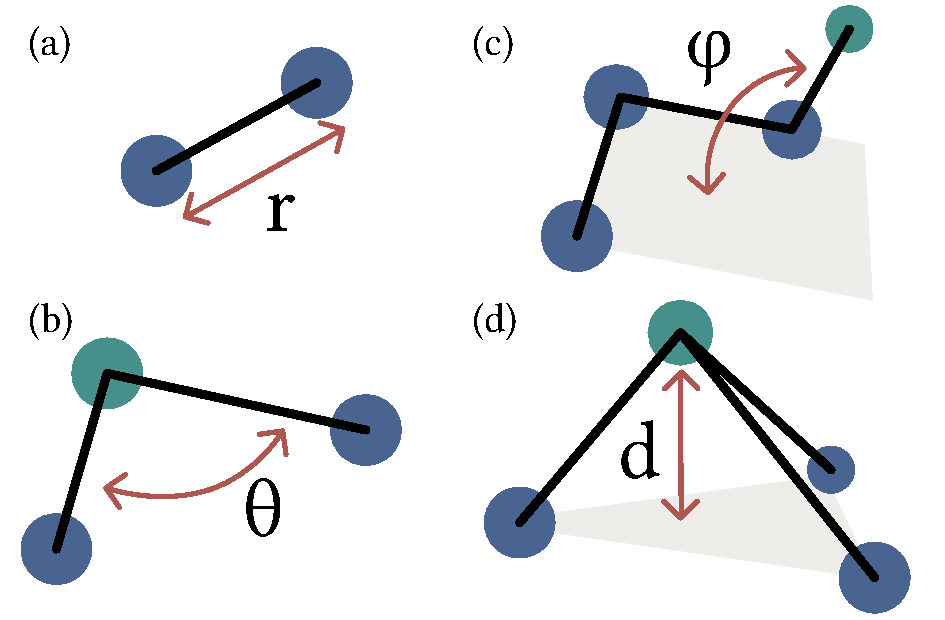
\includegraphics[width=.6\textwidth]{figures/images/molecular-ff}
    \caption{Definition of the parameters used to compute the energy of a
    molecular system with classical force field. (a) bond terms; (b) angle
    terms; (c) dihedral angles; (d) improper dihedrals/out of plane distance.}
    \label{fig:force-fields:molecular}
\end{figure}

\subsubsection{Typical functional forms used in force fields}

There is no strict rule regarding which functional form can or cannot be used in
a force field, so when creating a new force field we usually rely on chemical
sense as well as few physical laws to pick them. Bellow, I describe a few
well-known terms used in most force fields.

\textsc{Charges}\\[0.1\baselineskip]
If we choose to model atomic partial charges as point charges, we can directly
use the expression for Coulombic interactions, as a sum over all pairs of
charged atoms in the system:
\[ V(r_{ij}) = \frac{q_i q_j}{4 \pi \epsilon_0 r_{ij}}\]

It is also possible to use Gaussian charges distributions on each atom, where
the charge density around an atom is defined by a width parameter $\alpha_i$:
\[\rho_i = q_i \left(\frac{\alpha_i}{\sqrt\pi}\right)^3 e^{-\alpha_i^2 \ r_i^2}\]
In that case, the interaction between two atoms is given by --- using erf for
the error function:
\[ V(r_{ij}) = \frac{q_i q_j}{4 \pi \epsilon_0 r_{ij}}\ \text{erf}\left(\sqrt\frac{\alpha_i^2\alpha_j^2}{\alpha_i^2 + \alpha_j^2} \ r_{ij}\right)\]

I will discuss the issues that arise from using these type of potentials with
periodic boundary conditions, and the possible way to fix them such as Ewald
summation in section~\ref{sec:electrostatic}.

\textsc{Non-bonded pairs interactions}\\[0.1\baselineskip]
As we have seen, we use non-bonded pairs interactions to reproduce both the
Pauli repulsion between atoms at short distances, and the dispersion attractive
interaction at long distances. It can be shown\cite{London1930} that the
dispersion interaction can be developed in the long distances approximation as:
\[ V_\text{dispersion} = -\frac{C_6}{r^6} + \frac{C_8}{r^8} - \frac{C_{10}}{r^{10}} + \smallo\left(\frac{1}{r^{12}}\right) \]
where the $C_i$ coefficients have positive values. Most of the time, only the
term in $1/r^6$ is used, as it will have the largest contribution to the
resulting energy.

There is however no simple mathematical expression for the Pauli repulsion at
short distances, so various schemes have been used to approximate it. The most
prevalent one is the Lennard-Jones potential, which uses a repulsive term
proportional to $1/r^{12}$. In the early day of molecular simulation, this
allowed to save some computing time by squaring the already-computed $1/r^6$
term.
\[V_\text{Lennard-Jones}(r) = 4 \ \epsilon \left[\left(\frac{\sigma}{r}\right)^{12} - \left(\frac{\sigma}{r}\right)^6\right]\]
Another commonly used form is the Buckingham potential, using an exponential
function for the repulsion:
\[V_\text{Buckingham}(r) = A \ e^{-B r} - \frac{C}{r^6}\]

\textsc{Molecular interactions}\\[0.1\baselineskip]
The most common strategy for describing bonds and angles is to consider only
vibration of the bond length or the angle around the equilibrium, and represent
the energy of the bond/angle using the harmonic approximation:
\[V_\text{harmonic}(r) = \frac 12 k \ (r - r_0)^2 \qquad\text{or}\qquad V_\text{harmonic}(\theta) = \frac 12 k \ (\theta - \theta_0)^2 \]

For dihedral angles, we often want to be able to reproduce the periodicity of
the associated energy, which leads to the following definition of the energy:
\[V_\text{torsion}(\phi) = \frac 12 E \left[1 + \cos(n \phi + \delta)\right] \]

\subsubsection{Force field parametrization}

All these functional forms have one or more adjustable parameters, that depends
on the types of the atoms participating in the pair; bond; or angle. For
example, when using Coulombic interactions, the charge carried by an atom is the
adjustable parameter; when using a Lennard-Jones potential both the values of
$\sigma$ and $\epsilon$ are adjustable.

The process of adjusting these parameters to make sure the force field produces
the correct energy and physical properties of the system is called the
parametrization of a force field. It usually involves a trade-off between
accuracy --- \ie how well the force field can reproduce the potential energy
surface --- and transferability. A force field is said to be transferable if we
can use the same set of parameters for different systems. I will discuss it with
more depth in the next chapter, section~\ref{sec:classical-ff-parametrize}.

\subsection{System size and periodic boundary conditions}
\label{sec:pbc}

Everyday chemical systems contain a huge number of atoms, of the order of
Avogadro's number (\SI{e23}{} atoms). But when using molecular simulation to
study a chemical system, we are limited to a much smaller number of atoms: using
\SI{1}{TB} of computer memory we can only store positions and velocities for
around \SI{e10}{} atoms. This is even worse if we consider the number of atoms
for which we can compute properties with molecular simulation methods, of the
order of \SI{e4}{} to \SI{e7}{} atoms at most from today commodity hardware to
the biggest super-computers.

At these scales, the size and surface effects are not negligible: the surface
energy becomes an important part of the overall energy. The typical way to
remove these surface effects while keeping the number of simulated atoms low is
to use \emph{periodic boundary conditions}. The atoms are placed in a simulation
box called the \emph{unit cell}, which is replicated \emph{ad infinitum} in all
directions, as illustrated in figure~\ref{fig:pbc}.  The copies of the initial
box are called images of this box.

\begin{figure}[b]
    \centering
    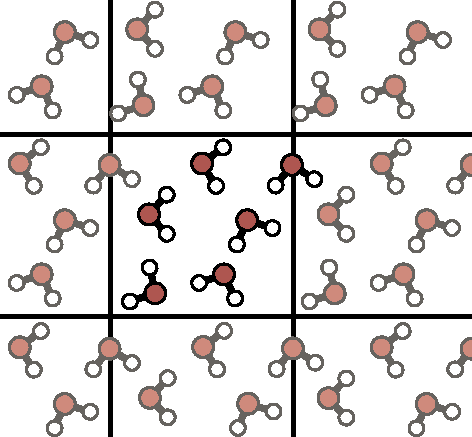
\includegraphics[width=0.6\textwidth]{figures/images/pbc}
    \caption{Illustration of periodic boundary condition in a two dimensional
    system. Molecules from the central cell are repeated in all directions.}
    \label{fig:pbc}
\end{figure}

In this arrangement, a molecule from the central simulation box will interact
with all molecules in the same box; but also with any molecule in any image
box, including with molecules image of itself. The effectively infinite
system created this way will not contain any surface effects, but other issues
can still affect the sampling and averaging of system properties.

First of all, the use of periodic boundary conditions introduces an artificial
periodicity into the system, which grows more important as the central
simulation box is smaller. For the study of crystalline materials, one has to
ensure that the periodicity of the simulation box matches the periodicity of the
crystal primitive cell. This periodicity also makes it harder to study defects
and other statistically rare features of the system. If we explicitly add a
defect to the system, it will be replicated over all the images, artificially
increasing the number of defects per unit of volume.

Second, because the system is now infinite, we need to compute an infinity of
interactions between molecules to evaluate its energy. Fortunately, most
interactions decay at long distances, and we can use a cutoff radius when
computing the energy. Any atoms further apart than this cutoff radius will not
interact. The error $\epsilon$ that arise from the use of a cutoff radius
$r_c$ depends on the potential $V(r)$ and the radial distribution function
$g(r)$ of the current conformation:
\[\epsilon(r_c) = \int_{r_c}^\infty r^2 V(r)\ g(r)\ \d r \]
If the cutoff radius is large enough (usually \SI{10}{\AA} is enough), then
$g(r) \simeq 1$ and we get a simpler estimation that does not depends on the
system conformation:
\[\epsilon(r_c) = \int_{r_c}^\infty r^2 V(r)\ \d r \]
For any function $V(r)$ that goes to zero at infinity faster than $1/r^3$, this
error is finite, and can be computed and applied afterward. Notably, the
electrostatic potential decays as $1/r$, and this error does not converge. In
order to describe electrostatic interactions properly in presence of periodic
boundary conditions, we need to use other methods such as the Ewald summation,
which I will present in more detail in section~\ref{sec:electrostatic}.

Finally, the \emph{minimum-image convention} is often used to improve simulation
speed. Under this convention, a particle in the central simulation box interacts
only with neighbors from the central image or an image surrounding the central
one. This restricts the number of images that has to be searched for neighbors
inside the cutoff radius. To be able to enforce this minimum-image convention,
the smallest inscribed sphere must have a radius bigger than the cutoff radius.
For an orthorhombic simulation box, the smallest box side length must be at least
twice the cutoff radius.

\newpage
\section{Metropolis Monte Carlo}

Now that we know how to compute the energy of any given configuration, our goal
of computing macroscopic properties from microscopic states is getting closer.
The idea is to evaluate the integral in equation~\eqref{eq:observable} by using
a finite set of configurations $\{\r^N\}_\alpha$ distributed according to the
right distribution, which depends on the ensemble. The ensemble average
$\braket{A}$ of a property $A$ that only depends on the spatial conformation of
the system gives us the value of this property at the macroscopic level:
\[\braket{A} \approx \frac 1 m \sum_\alpha^m A(\r_\alpha^N) \label{eq:mc:sampling}\]

Metropolis Monte Carlo is an algorithm that enables us to generate new
configurations following a given distribution, using only an initial
configuration of the system. This means that we can directly sample the ensemble
of interest.

\subsection{The basic algorithm}

\begin{figure}[ht]
    \centering
    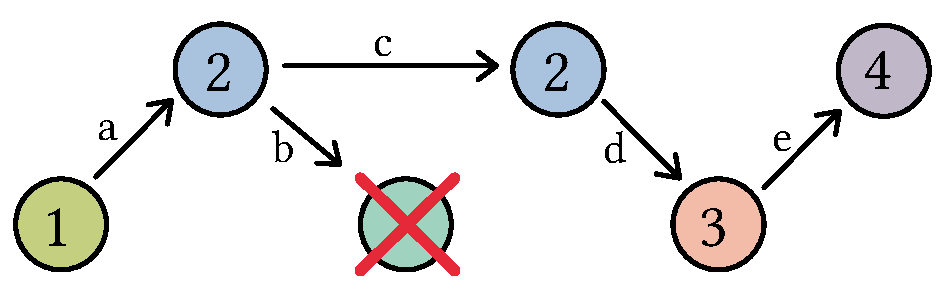
\includegraphics[width=0.6\textwidth]{figures/images/mc-chain}
    \caption{Illustration of a Markov chain in Metropolis Monte Carlo.
    Configurations are numbered from 1 to 4, and letters from (a) to (e) are used
    for tentative moves. Step 2 appears twice in the chain, as the tentative
    move (b) was rejected.}
    \label{fig:mc:chain}
\end{figure}

The Metropolis Monte Carlo method is part of the family of Markov Chain Monte
Carlo algorithms. A Markov chain is a set of configurations, such that the
probability of generating a new configuration only depends on the previous
configuration of the chain: it has no further \emph{memory} of older states. A
Markov chain is thus completely defined by the knowledge of the initial state
and the procedure used to generate a new state.

When using a Markov chain to explore and sample the phase space, we want it to
be able to explore all the possible states in the phase space. In order to
ensure this, we want the chain to be \emph{ergodic}, \ie that each state can be
reached from any other state in a finite number of steps. This property
guarantees the existence of a \emph{stationary} equilibrium distribution of the
generated states as the Markov chain grows, and that this distribution matches
the probability to generate a new state from any given state. For us, this means
that if we are able to create an ergodic Markov chain using the Boltzmann
statistics to generate a new state, then the whole chain will follow the
Boltzmann distribution. The same reasoning also works in other statistical
ensembles, following their own distribution of probability.

\subsubsection{Micro-reversibility}

The usual way to ensure we have an ergodic Markov chain is to impose that this
chain is \emph{micro-reversible}. Although this is not a required condition to
have an ergodic chain, it is a sufficient one\cite{Frenkel2002}, and quite
commonly used. Using $\mathcal{P}_i$ for the probability of being in a state
$i$, and$\pi(i \to j)$ the probability to go from state $i$ to state $j$, the
condition of micro-reversibility is defined as:
\[ \mathcal{P}_i \ \pi(i \to j) = \mathcal{P}_j \ \pi(j \to i)\]
This means that the probability for any transition in the Markov chain to be
from state $i$ to state $j$ must be the same as the probability for this
transition to be from state $j$ to state~$i$. In Metropolis Monte Carlo, the
generation of a new state is a two-step process: first we generate a new
configuration, and then we accept or reject this new configuration. If we accept
the configuration, then the new state of the Markov chain is the new
configuration; else the new state of the chain is the old configuration. This is
illustrated in figure~\ref{fig:mc:chain}. This makes the probability $\pi(i \to
j)$ a product of the probability $\alpha(i \to j)$ to generate a given new
configuration and the probability $\text{acc}(i \to j)$ to accept it.
\[\pi(i \to j) = \alpha(i \to j)\times\text{acc}(i \to j)\]

The original Metropolis scheme\cite{Metropolis1953} chooses the $\alpha$
probability to be symmetric, \ie $\alpha(i \to j) = \alpha(j \to i)$, the
probability of generating a configuration $j$ from $i$ is the same as the
probability of generating the configuration $i$ starting from $j$. This gives us
\[ \frac{\text{acc}(i \to j)}{\text{acc}(j \to i)} = \frac{\mathcal{P}_j}{\mathcal{P}_i} \label{eq:mc:acceptance}\]
We want to set the resulting probability of the Markov chain to follow Boltzmann
statistics, which gives us
\[ \frac{\text{acc}(i \to j)}{\text{acc}(j \to i)} = e^{-\beta [U(j\,) \;-\; U(i\,)]} \]
There are multiple choices that would result in this same relation. The standard
choice is to always accept the transition from $i$ to $j$ if the energy
decreases ($\Delta U = U(j\,) - U(i\,) < 0$), or else accept it with probability
$e^{-\beta \Delta U}$.
\[\text{acc}(i \to j) = \min\left[1, \exp\left(-\beta \Delta U\right)\right] \label{eq:mc:acceptance:nvt}\]

In order to accept a configuration change with probability $e^{-\beta \Delta U}$,
we usually generate a random number $r$ with uniform distribution in $[0, 1]$,
and accept the new configuration if $r < e^{-\beta \Delta U}$.

When working in ensembles other than the canonical ensemble, we can still
apply the same procedure, simply changing the acceptance probability to agree
with the required distribution. For example, in the $NPT$ ensemble, the
probability to be in a state is proportional to $e^{-\beta\, U(\r) \; - \; \beta PV}$.
This changes the acceptance probability to
\[\text{acc}^{NPT}(i \to j) = \min\left[1, \exp\left(-\beta \Delta U - \beta P \Delta V \right)\right]\label{eq:mc:acceptance:npt}\]

\subsection{Monte Carlo moves}

\begin{figure}[t]
    \centering
    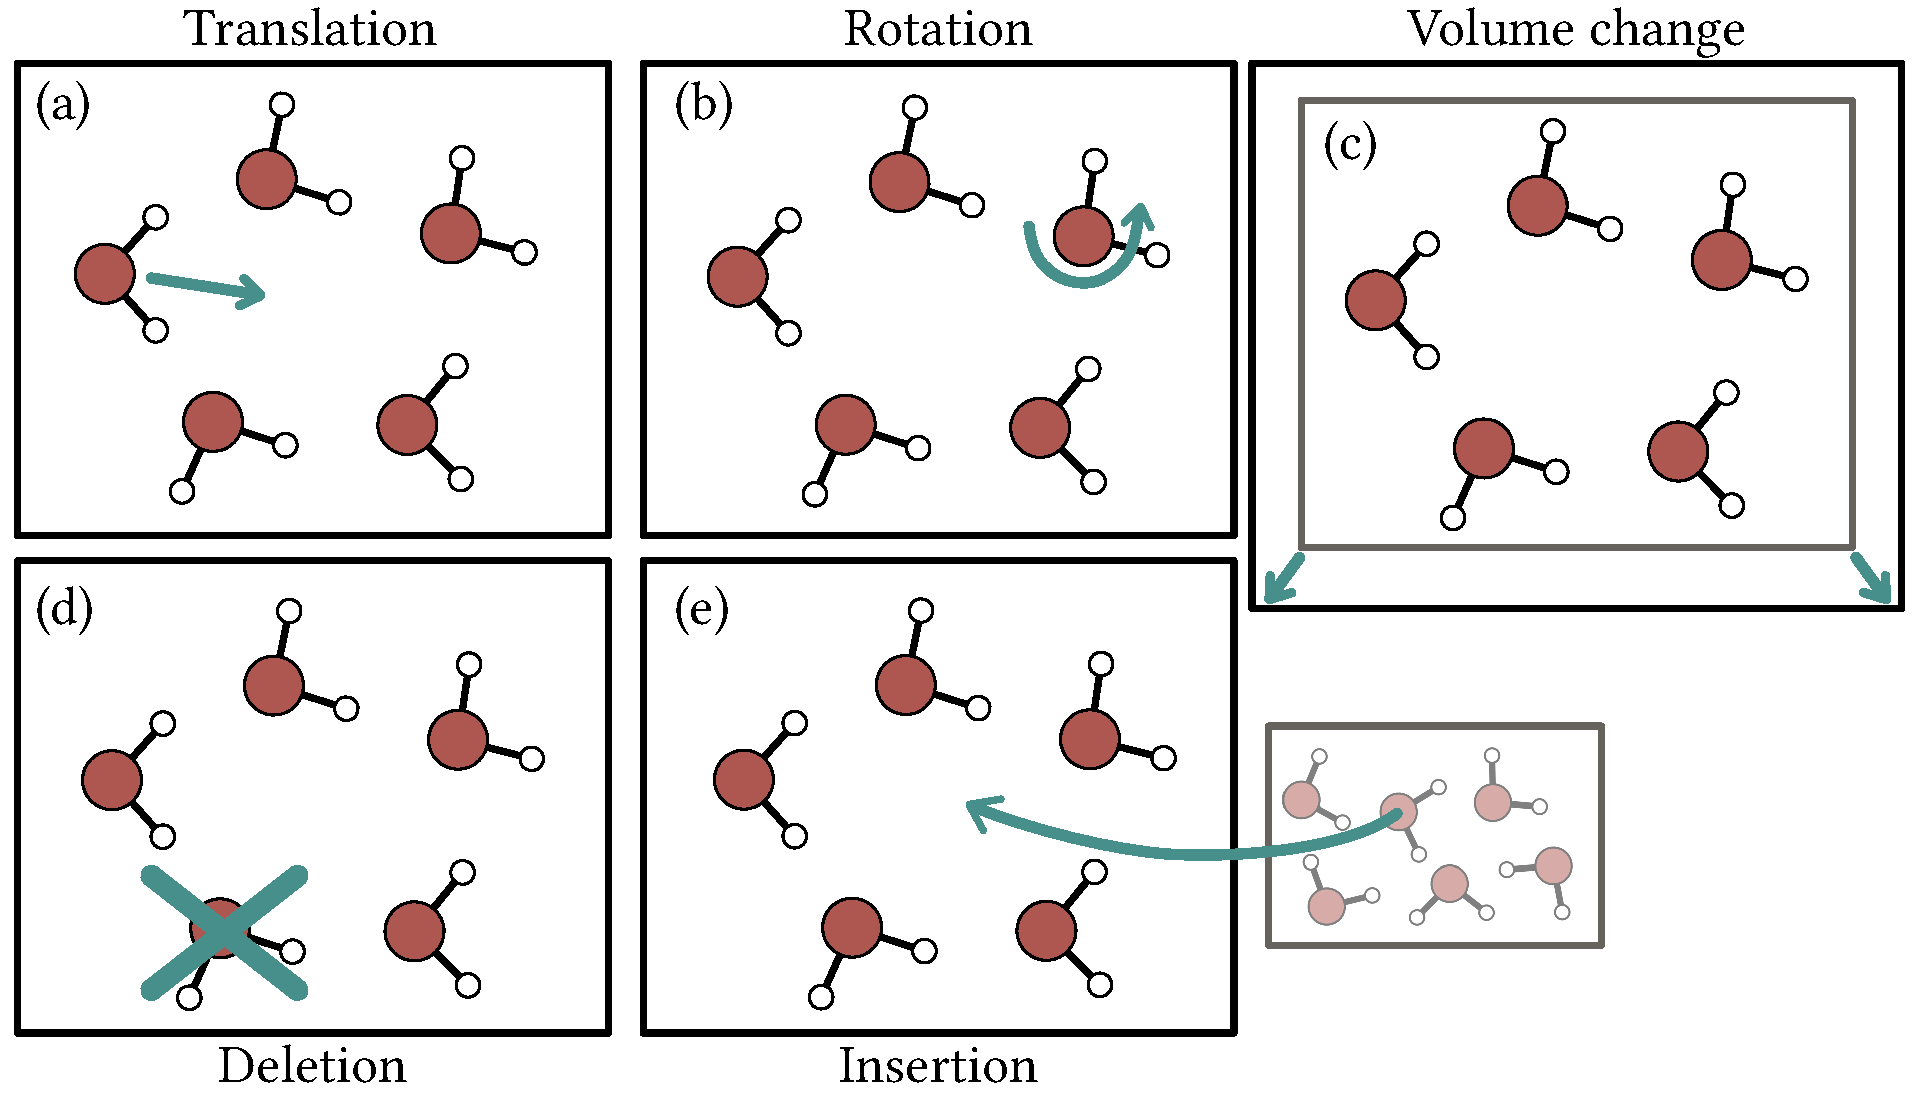
\includegraphics[width=0.8\textwidth]{figures/images/mc-moves}
    \caption{Basic Monte Carlo moves: (a) translation of a single molecule; (b)
    rotation of a single molecule; (c) unit cell volume change; (d) molecule
    deletion; (e) molecule insertion from a reservoir.}
    \label{fig:mc:moves}
\end{figure}

The last remaining piece of the puzzle before being able to run Monte Carlo
simulations is to specify a way to generate new configurations. We need to
construct them such that the probability of creating a state $j$ from $i$ is the
same as creating the state $i$ starting from $j$; \ie $\alpha(i \to j) =
\alpha(j \to i)$. In implementations of Metropolis Monte Carlo for molecular
simulation, basic algorithms used to generate a new conformation from the
previous one are called \emph{moves}. At each step of the simulation, a specific
move is selected at random in the list of possible moves, ensuring $\alpha(i \to
j) = \alpha(j \to i)$ globally as long as the move itself enforce $\alpha(i \to
j) = \alpha(j \to i)$.

\subsubsection{Canonical ensemble: translations and rotations}

The simplest move imaginable is to randomly select an atom and move it by a
random distance in a random direction. The newly generated state only differs
from the previous one by the position of this atom. When working with rigid
molecules, this move can also be used to translate a full molecule. But in that
case, we also need to account for rotational degrees of freedom. We use random
rotations (random rotation axis and magnitude) of molecules to do so. These
moves are illustrated in figure~\ref{fig:mc:moves}, panels (a) and (b). By using
uniform distributions for the cartesian components of the translation, the
amplitude of the rotation, and uniform sampling of the unit sphere for the
rotation axis; these moves have the same probability of going from a state $i$
to $j$ and vice versa.

The one remaining parameter is then the amplitude of the move, \ie the interval
in which to draw the translation or rotation amplitude with a uniform
distribution. It is desirable to have an acceptance rate around 40 to 50\%, as a
lower acceptance rate means that we are wasting computation time to generate
conformations that will not be used, and a higher acceptance rate usually means
that the new conformation will be very close to the previous one, and the
simulation will take longer to sample the phase space. We can adjust the
amplitude of the rotations and translations to influence the value of
$\alpha(i \to j)$: larger amplitude means a smaller acceptance rate, and smaller
amplitude means a higher acceptance rate. But adjusting the amplitude breaks
micro-reversibility, and as such should be done beforehand to prevent affecting
the simulation results. It is thus customary to break a simulation in two
phases: a first equilibration phase to adjust the simulation parameters, and a
later production phase that will be used for statistical analysis and averaging.

Translations and rotations, together with the acceptance scheme defined in
equation~\eqref{eq:mc:acceptance:nvt}, are enough to generate a Markov chain
sampling the $NVT$ ensemble. The temperature of the system is set by the value
of $\beta$ used in equation~\eqref{eq:mc:acceptance:nvt}, and the number of
particles and volume are set by the initial conformation. The conformations in
the Markov chain can then be used with equation~\eqref{eq:mc:sampling} to
evaluate the macroscopic properties of the system.

\subsubsection{Isobaric-isothermal ensemble: volume changes}

If we want to work in another thermodynamic ensemble such as the $NPT$ ensemble,
we need first to change the acceptance scheme to
equation~\eqref{eq:mc:acceptance:npt}, and also to generate moves that change
the system's volume. One way to change the volume is to randomly pick a new
volume using a uniform distribution centered around the old volume, and then
resize the simulation unit cell while keeping intra-molecular distances
constant. This is illustrated in figure~\ref{fig:mc:moves}, panels (c). Keeping
the distances constant ensures that the change in energy $\Delta U$ will not be
too big, and that the move will be accepted more often than with a simple
scaling scheme. As for translations and rotations, we can adjust the acceptance
rate of the move by changing the amplitude of volume changes.

\subsubsection{Grand Canonical ensemble: insertion and deletion}

Simulations in the $\mu VT$ ensemble are called Grand Canonical Monte Carlo
(GCMC) simulations. In this ensemble, the number of molecules is allowed to
fluctuate in order to maintain the chemical potential constant. We need two
moves to accomplish this, one where we select a molecule at random and remove
it, and another one where a molecule is inserted from a fictitious reservoir at
a random position and orientation (see figure~\ref{fig:mc:moves}, panels (d) and
(e)). The acceptance probability is given as previously by the $\mathcal{P}_j /
\mathcal{P}_i$ ratio; but this time the $N!\ \lambda^{3N}$ terms from
equation~\eqref{eq:probably:uvt} do not cancel out. For the insertion of a new
molecule we have:
\[ \text{acc}(N \to N + 1) = \min\left[1, \frac{V}{\lambda^3 (N + 1)} \exp\left(\beta \mu - \beta \Delta U \right)\right]; \]
and for the removal of a molecule,
\[ \text{acc}(N \to N - 1) = \min\left[1, \frac{\lambda^3 N}{V} \exp\left(-\beta \mu - \beta \Delta U \right)\right]. \]

Unfortunately, the chemical potential $\mu$ is not easily known before starting
a simulation and these expressions are hard to use. Instead, for chemical
species in the gas phase we use the fugacity $f$ of the gas, defined as the
pressure of an ideal gas with the same temperature and molar free enthalpy as
the real gas. It is related to the chemical potential by $f = e^{\,\beta \mu} /
\beta \lambda^3$.  Replacing in the equation above gives us the standard
acceptance probabilities for GCMC simulations in the gas phase:
\begin{gather}
\text{acc}(N \to N + 1) = \min\left[1, \frac{\beta V f}{N + 1} \exp\left(- \beta \Delta U \right)\right] \\
\text{acc}(N \to N - 1) = \min\left[1, \frac{N}{\beta V f} \exp\left(- \beta \Delta U \right)\right]
\end{gather}

For other phases such as liquids, the relation between chemical potential and
pressure $\mu(P)$ for the bulk phase has to be established first, by separate
series of Monte Carlo simulations.

\subsection{Monte Carlo caveats}

Monte Carlo simulations are very powerful, as they allow to directly sample the
phase space of the ensemble of interest, and do not require that the moves used
to generate a new trial configuration follow the laws of physics. This later
property is used in some extensions of Monte Carlo simulations, where an atom
nature is transformed as a Monte Carlo move, changing a sodium atom into a
potassium atom for example. This method --- called semi-grand canonical Monte
Carlo\cite{Kofke1988} --- allows to sample the equilibrium distribution during
chemical reactions or at an interface without explicitly representing the
interface.

They also have a few caveats, mainly it is not possible to sample the
microcanonical  ensemble, as this would require generating trial configurations
with constant energy, and updating both the positions and velocities of the
atoms. The main problem with Monte Carlo simulation is that they only deal with
the conformations of the system, and do not contain any information on the
kinetics of the transformations. Both of these caveats can be solved by using
molecular dynamics instead to generate the states used to evaluate
equation~\eqref{eq:observable}.

\begin{figure}[b]
    \centering
    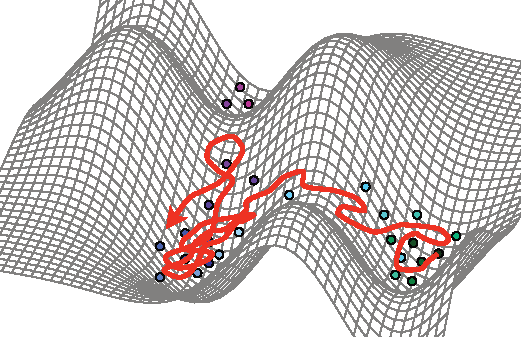
\includegraphics[width=\textwidth]{figures/images/mc-vs-md}
    \caption{Representation of the way the potential energy surface is explored
    by molecular dynamics (red line) and Monte Carlo (colored circles)
    simulations.}
    \label{fig:mc-vs-md}
\end{figure}

\clearpage
\section{Molecular dynamics}
\label{sec:molecular-dynamics}

The fundamental idea of molecular dynamics is to use Newton's laws of motion to
integrate the positions and velocities of the atoms in the system as a function of
time. In this work, I will consider that the atoms in the system behave as
classical point particles. There are multiple methods to go beyond this
approximation and incorporate the quantum nature of atoms, mostly based on
Feynman path integrals\cite{Craig2004}.

Newton's laws give us differential equations on the time evolution of positions
and velocities ($\p_i = m_i \v_i$):
\[\frac{\partial \r_i}{\partial t} = \v_i; \qquad\text{and}\qquad m_i \frac{\partial \v_i}{\partial t} = - \frac{\partial U(\r)}{\partial \r_i}. \]
We can discretize time in these equations by considering a succession of
instants separated by the \emph{time step} $\delta t$. If we then replace the
derivatives with first order finite differences, we get the Euler integrator
equations:
\[ \r_i(t + \delta t) = \r_i(t) + \v_i(t) \delta t + \smallo(\delta t^2)\]
\[ \v_i(t + \delta t) = \v_i(t) + \frac{1}{m_i} \vec f_i(t) \delta t + \smallo(\delta t^2) \]
where $\vec f_i =\kern-0.7ex - \partial U(\r) / \partial \r_i$ is the force
acting on atom $i$. The Euler integration scheme presented here have a high
discretization error and is not used in actual simulations, but helps
understanding molecular dynamics. Better integration schemes will be presented
below.

Starting from an initial configuration defined by the positions and velocities
of each atom at time $t$, these equations allow to compute the positions and
velocities at the next time point $t + \delta t$. For this discretization to be
valid, the time step $\delta t$ has to be small enough so that both the
$\smallo(\delta t^2)$ terms are negligible, and the forces acting on each atom
are constant between $t$ and $t + \delta t$. Depending on the system, typical
values for the time step fall between \SI{0.5}{fs} and \SI{2}{fs}.

Time integration of positions and velocities follows the standard rules of
classical mechanics, and in particular the conservation of mechanical energy.
This means that by default, molecular dynamics trajectories evolve in the
microcanonical  $NVE$ ensemble. There however is no \emph{a priori} guarantees
that a molecular dynamics trajectory will generate new configurations following
the microcanonical  distribution. We rely on the \emph{ergodic} hypothesis to
assume that the trajectory does sample the whole $NVE$ ensemble. In the most
intuitive form, this hypothesis is formulated as:

\vskip0.8ex
\begin{quote}
    At equilibrium, the ensemble average of a property is the same as the
    average of the values of this property taken over a high number of
    measurements in different points in time.
\end{quote}
\vskip0.8ex

The ergodic hypothesis links together the statistical physics view of the world,
and what can effectively be measured at the macroscopic level. Mathematically
speaking, the ergodic hypothesis is a property of the Hamiltonian system: a
system is said to be ergodic if the point representing this system in the phase
space can approach every point in the phase space as closely as desired. In this
case, the Birkhoff ergodic theorem proves that the time average and ensemble
average are the same almost everywhere. This condition has been verified for
some systems, and is usually assumed to hold when working with statistical
thermodynamics.

\subsection{Integration schemes}

\subsubsection{Desirable properties}

We want the integration scheme used for a molecular dynamics simulation to
enforce the symmetry and conservation properties of a real mechanical system;
namely the time reversal symmetry, conservation of energy, linear momentum,
angular momentum and phase space volume. Conservation of phase space volume is a
consequence of  Liouville's theorem concerning the phase space distribution
$\rho(\r^N, \v^N)$:
\[\frac{\d \rho}{\d t} = \frac{\partial \rho}{\partial t} + \sum_i \left(\frac{\partial \rho}{\partial \r_i} \frac{\d \r_i}{\d t} + \frac{\partial \rho}{\partial \v_i} \frac{\d \v_i}{\d t} \right) = 0.\]
This means that if we consider a set of initial conditions inside a closed and
bounded region of phase space and propagate them for a given time, the resulting
points in phase space will still be a closed and bounded region of phase space
with the same volume as the initial region --- this is illustrated in
figure~\ref{fig:symplectic-integrator}. An integrator conserving the phase space
volume is said to be \emph{symplectic}.

\begin{figure}[ht]
    \centering
    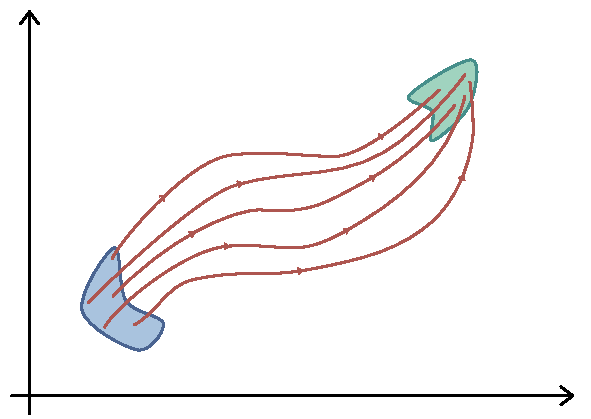
\includegraphics[width=0.7\textwidth]{figures/images/symplectic-integrator}
    \caption{Illustration of a set of trajectories (in red) in a 2 dimensional
    phase space. For a symplectic integrator, the initial volume (in blue) will
    be the same as the final volume (in green).}
    \label{fig:symplectic-integrator}
\end{figure}

Because we are approximating the equations of motion by evaluating them on
discrete time steps the energy might not be fully conserved, and an energy drift
can appear. The amplitude of this drift will depend on the choice of time step;
a bigger time step will introduce a bigger error. Good integrators will allow us
to use bigger time steps while keeping the drift small. In turn, this makes the
overall simulation more efficient by reducing the number of steps needed to
simulate long processes. Another way to make the simulation more efficient is to
evaluate the forces acting on the atoms as rarely as possible. This is the case
in multi-timesteps methods such as reversible Reference System Propagator
Algorithms\cite{Tuckerman1992} (r-RESPA) where forces are separated by the time
scale of their variations, and evaluated only when needed instead of being
calculated at all steps.

\subsubsection{Some examples of integration schemes}

One of the simplest integrator respecting all the above defined constraints
(symplectic, time-reversible, energy conservation) is the \emph{leap frog}
integrator\cite{Frenkel2002}. The corresponding algorithm is reproduced below,
using $\r(n)$ for $\r(n \times \delta t)$, and $\vec f(n)$ for the forces
computed from the positions at step $n$.
\[\begin{aligned}
    \vec a(n)   &= \frac{1}{m}\ \vec f(n), \\
    \v(n + 1/2) &= \v(n - 1/2) + \vec a(n) \,\delta t, \\
    \r(n + 1)   &= \r(n) + \v(n + 1/2)\,\delta t,
\end{aligned}\]

Evaluation of the forces is made clear by the $a = f / m$ line, to ensure it
only occurs once. The leap frog integrator is more stable than the previously
mentioned Euler integrator. Unfortunately, it computes the positions and
velocities at interleaved instants, staggered in such a way that they jump over
each other in a frog-like fashion.

Velocity-Verlet integrator fixes this issue while keeping the symplectic and
time reversible nature of leap frog\cite{Verlet1967, Frenkel2002}. The algorithm
works as follow:
\[\begin{aligned}
    \v(n + 1/2)   &= \v(n) + \frac 12 \vec a(n)\,\delta t, \\
    \r(n + 1)     &= \r(n) + \v(n + 1/2)\,\delta t, \\
    \vec a(n + 1) &= \frac{1}{m}\ \vec f(n + 1), \\
    \v(n + 1)     &= \v(n + 1/2) + \frac 12 \vec a(n + 1)\,\delta t,
\end{aligned}\]
Here, velocities are updated twice by a half step, but the forces are still
computed only once. This algorithm also yields the positions and velocities at
full time steps, allowing them to be used together when computing properties of
the system.

Both integrators presented here have a $\smallo (\delta t^2)$ error, but they
are other integration scheme with a smaller error, called higher-order
integrators. The most famous ones are the Runge–Kutta methods, that can be
derived for any even order, starting with $\smallo (\delta t^4)$. Runge–Kutta
integrators are not used as often as the Velocity-Verlet or leap frog
integrators, as they are more expensive to use and are not time-reversible.

\subsection{Sampling other ensembles}

By default, molecular dynamics samples the $NVE$ ensemble since the mechanical
energy, volume and number of particles are kept constant. To sample another
ensemble, we need a way to control the variable that changes from this ensemble
to the $NVE$ ensemble. For example, going from $NVE$ to $NVT$, we want to
change the energy of the system as $E$ and $T$ are conjugated variables.
Similarly, going from $NVT$ to $NPT$ requires changes to the volume.

\subsubsection{Thermostats}

Algorithms that control the temperature by changing the energy of the system are
called \emph{thermostating} algorithms, or \emph{thermostats} for short.  They
work by changing the kinetic energy of the system, or more generally by changing
the velocities of the atoms. As illustrated in figure~\ref{fig:thermostats},
for the same system,  different thermostats will produce different temperature
response.

In the simplest (and crudest) approach, if we want to change the system
temperature from $T_0$ to $T_1$, we need to multiply all velocities by
$\sqrt{T_1 / T_0}$. As the system evolves, the temperature needs to be updated
again, as kinetic energy is transferred into potential energy and reciprocally
by the integrator. This approach is sometimes called a \emph{rescaling}
thermostat. While this algorithm does fix the system temperature to the target
value, the integrator is no longer time-reversible and symplectic. This also
introduces many non-physical artifacts in the dynamics. One example of such
non-physical effect is the so-called \emph{flying ice cube}; where all the
thermal energy of the system is transferred into the global translation
velocity, while removing all vibrational energy from the atoms, resulting in a
simulation of flying frozen atoms.  Finally, the simulation does not sample the
true $NVT$ ensemble, since the kinetic energy is not allowed to fluctuate around
its equilibrium value.

The \emph{weak coupling} or Berendsen\cite{Berendsen1984} thermostat is a
slightly better version of the rescaling thermostat that imposes a first-order
(exponential) relaxation of the temperature such that
\[\frac{\d T(t)}{\d t} = \frac{T_0 - T(t)}{\tau_T};\]
where $T(t)$ is the instantaneous system temperature, $T_0$ the target external
temperature, and $\tau_T$ the relaxation time constant. The instantaneous
temperature is computed from the system's kinetic energy $E_\text{kin} = \sum_i
m_i \v_i^2(t) $ as
\[T(t) = \frac{2 \ E_\text{kin}(t)}{n_f\ k_B},\]
where $n_f$ is the number of degrees of freedom in the system, $3 * N$ for fully
flexible molecules. The Berendsen thermostat is implemented by rescaling the
velocities at each time step by
\[\alpha = \sqrt{1 + \frac{\delta t}{\tau_T} \left(\frac{T_0}{T(t)} - 1\right) }.\]
The Berendsen thermostat models a system weakly coupled to a heat bath at
temperature $T_0$. In order to sample the canonical ensemble, we need an
algorithm that is able to reproduce both the average value of the temperature
and the fluctuations around the equilibrium of this temperature. Because it
diminishes fluctuations of the kinetic energy of the system, the Berendsen
thermostat is unable to produce trajectories in the canonical $NVT$
ensemble\cite{Braun2018}. It is still useful for the equilibration phase of a
simulation, where one wants the system to reach approximate equilibrium as fast
as possible.

To probe the correct canonical ensemble, we can instead use a
Nosé-Hoover\cite{Nose1984,Hoover1985} thermostat. In this approach, the
Lagrangian (and thus the Hamiltonian) of the system is modified to include an
additional variable $s$ controlling the temperature of the system by changing
the time scale of the extended system such that $\delta t' = s\, \delta t$. This
new variable is coupled to the system by changing all the velocities to $\v' =
s^{-1}\ \d \r / \d t$. It can be shown that sampling the extended system in the
microcanonical  ensemble is equivalent to sampling the real system in the
canonical ensemble, including the fluctuations. The intensity of the coupling is
can be tuned by changing the fictitious mass associated with $s$. The extended
Lagrangian can be propagated through time with any existing time-reversible and
symplectic integrator.

Instead of using such extended Lagrangian methods, it is also possible to modify
the rescaling methods to sample canonical ensemble. This is the basis of the
Canonical Sampling through Velocity Rescaling\cite{Bussi2007} (CSVR) thermostat
which I also used during my PhD. The main idea is to replace the $\alpha$
scaling parameter from Berendsen thermostat by a parameter picked randomly using
the expected distribution for the fluctuations of kinetic energy. The trajectory
will then explore the canonical ensemble, by construction.

\begin{figure}[ht]
    \centering
    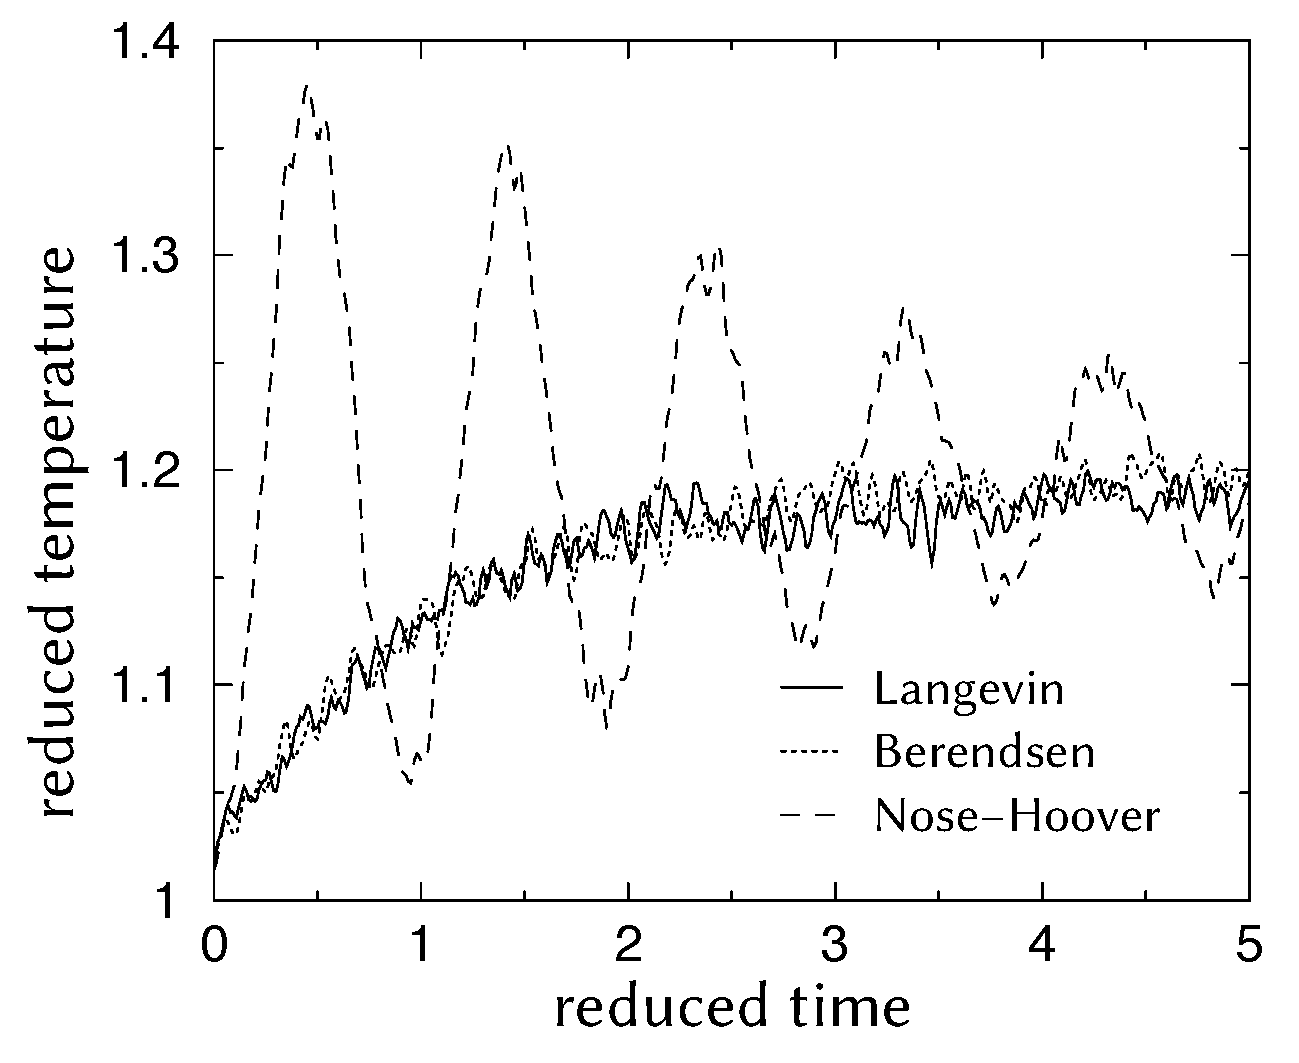
\includegraphics[width=0.7\textwidth]{figures/images/thermostat-response}
    \caption{The temperature response of a Lennard–Jones fluid under control of
    three thermostats (solid line: Langevin, not presented here; dotted line:
    Berendsen; dashed line: Nosé–Hoover) after a step change in the reference
    temperature. Image adapted from reference~\cite{Hess2002}.}
    \label{fig:thermostats}
\end{figure}

\subsubsection{Barostats}

Controlling the pressure can be done with the same approaches as the temperature
to generate the $NPT$ ensemble. In this case, we want to fix the value of the
pressure $P$ by dynamically changing the volume $V$ of the system. For example,
the Berendsen barostat\cite{Berendsen1984} rescales the system volume at every
step to ensure first-order relaxation to the target pressure. For a cubic unit
cell subject to isotropic pressure, this means multiplying the cell volume by
\[ \eta(t) = 1 - \frac{\beta\,\delta t}{\tau_P} \left(P_0 - P(t)\right);\]
where $P_0$ is the target pressure, $P(t)$ the instantaneous system pressure,
$\tau_P$ the pressure relaxation time constant and $\beta$ the compressibility
of the system; often approximated by the compressibility of liquid water. We
then multiply the atomic positions by $\sqrt[3]{\eta}$. If the system is subject
to an anisotropic stress tensor $\underline{S}_0$, then the unit cell matrix
should be resized by:
\[ \underline{\eta} = \mathds{1} - \frac{\beta\,\delta t}{\tau_P} \left(\underline{S}_0 - \underline{S}(t)\right). \]

As for thermostats, the Berendsen barostat does not sample the actual
isothermal-isobaric ensemble, as it cannot accurately reproduce the volume
fluctuations of the $NPT$ ensemble. It is still very useful for system
equilibration when starting a simulation. The Nosé-Hoover barostat is based on
an extended Lagrangian, and can sample the real $NPT$
ensemble\cite{Tuckerman2010}. To my knowledge, there is no equivalent to the
CSVR thermostat for controlling the pressure.

When using both a thermostat and a barostat to control the system pressure and
temperature, one must take care that both control algorithms have sufficient
time to react to changes. In particular, every time the barostat changes the
simulation cell, the thermostat must change the velocities to adapt the kinetic
energy to the new potential energy. This means that the time step used for the
barostat should be higher than the one used by the thermostat. In my
simulations, I found that setting $\tau_P = 10 \times \tau_T = 1000 \times \Delta
t$ works well in practice.

\subsubsection{Can osmostats exist? Grand canonical molecular dynamics}
\label{sec:gcmd}

As we have seen, it is possible to go from an ensemble to another by
controlling the conjugated variables: change $E$ to control $T$, $V$ to control
$P$. It is then natural to consider whether it is possible to control the
chemical potential of a system to sample the grand canonical $\mu V T$
potential. The obvious way to do so is to change the number of particles in the
system. Multiple versions of such \emph{Grand Canonical Molecular Dynamics} have
been presented over the years, either using an extended Hamiltonian
approach\cite{Cagin1991,Lo1995,Eslami2007}, or a mixture of Monte Carlo moves
and molecular dynamics integration in the same
trajectory\cite{Heffelfinger1994,Cracknell1995,Boinepalli2003}.

The latter methods --- mixing Monte Carlo moves with molecular dynamics
integration --- have not been proven, to my knowledge, to generate any specific
statistical ensemble. While Monte Carlo simulations and molecular dynamics are
proven to do so under certain hypotheses, we lack such mathematical proofs for
the generic hybrid case. It is possible to mix molecular dynamics and Monte
Carlo under the framework of Hybrid Monte Carlo simulations, which I will
discuss in more details in chapter~\ref{sec:hmc}. The main idea here is to use
short Molecular Dynamics simulations as a new Monte Carlo move to generate new
configurations. Under some conditions on the molecular dynamics integrator, the
resulting Markov chain is proven to be ergodic. In this case, the simulation is
a Monte Carlo simulation, and not a molecular dynamics one: Molecular dynamics
is only used as a mean to generate new configurations, and the underlying
trajectory is thrown away. Because of this, the resulting simulation suffers
from the same limitations as all Monte Carlo simulations, and in particular the
absence of any dynamic information.

For the methods using an extended Hamiltonian approach, the general idea is to
have one or more \emph{fractional} particles in the system, represented by a
parameter $\lambda$ going from 0 to 1.  The interactions of this particle with
the system are scaled down by $\lambda$, and the value of $\lambda$ evolves
through time. When it reaches 1, the particle is converted to a full particle
and a new one is inserted with a small $\lambda$, and when it reaches 0, the
particle is removed and a new one is picked to have the value of $\lambda$
change.

This approach has several limitations, starting with the fact that
time-reversibility is broken when $\lambda$ reaches 0 or 1. Additionally,
Liouville's theorem (the fact that the phase-space distribution function is
constant along the trajectories of the system) is only proven for a constant
number of atoms, and might not be valid in the grand canonical
ensemble\cite{DelleSite2016}. This can be understood intuitively: in both $NVE$,
$NVT$ and $NPT$ simulations, the system explores a certain sub-space of the
phase space, the hyper-surfaces at a constant energy/temperature, or the
hyper-volume at constant pressure respectively. In the grand canonical ensemble,
the underlying number of dimensions of the ensemble would change depending on the
position in the extended phase space. As all of our current theory and
understanding of Hamiltonian dynamics is based on a constant number of
particles, using molecular dynamics to sample the grand canonical ensemble might
not be possible. Fortunately, we can still use Grand Canonical Monte Carlo for
this.

\subsection{Molecular dynamics caveats}

The main advantage of molecular dynamics simulations is the explicit description
of time. This allows to study time-dependent phenomena, and make the simulation
trajectories easier to interpret as they form a "movie" of what is happening in
the system.

But these simulations also have a few limitations. As they are based on
Hamiltonian dynamics, they can only sample ensembles with a constant number of
particles.  At the same time, it is harder to ensure that the trajectory is
sampling the right ensemble, compared with Monte Carlo simulations where the
ensemble is built directly into the moves and their probabilities. Generating
the right average value --- for example when using a Berendsen thermostat --- is
not enough, and one must check that the full distribution is reproduced.

In general, Monte Carlo and molecular dynamics simulations complete each other,
one having strengths where the other is weaker, or harder to use. The main
difference between them remains the way they explore the phase space,
represented figure~\ref{fig:mc-vs-md}. Molecular dynamics will generate a smooth
trajectory in the phase space, while Monte Carlo trajectories will exhibit jumps
and discontinuities. This ability to use non-physical moves (such as a change
in the number of particles in the system) make Monte Carlo simulations a more
versatile tool for molecular simulations, able to jump over local energy
barriers and improve sampling rate of the phase space.

\newpage
\section{Free energy methods}

\begin{figure}[ht]
    \centering
    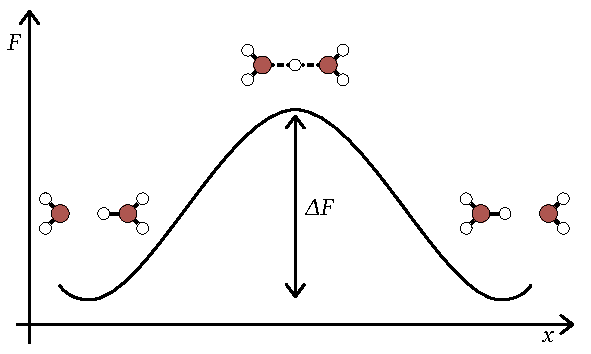
\includegraphics[width=0.7\textwidth]{figures/images/free-energy-profile}
    \caption{Representation of a free energy profile along a reaction
    coordinate $x$, on the example of proton exchange in water.}
    \label{fig:free-energy-profile}
\end{figure}

Sometimes, the knowledge and sampling of the whole phase space is not necessary
to acquire insight into the system of interest. For example, a reaction occurring
in a water solution will only involve a few degrees of freedom (the distance
between the reacting molecules) among the thousands of degrees of freedom
composing the phase space --- this is illustrated in
figure~\ref{fig:free-energy-profile} where the distance of the proton to the
first water molecule is used as reaction coordinate. In these cases, it
can be more efficient to only consider these degrees of freedom and extract the
corresponding free energy surface. This is what free energy methods are designed
to do. The idea is to bias the system to sample preferentially the degrees of
freedoms of interest, and extract the free energy profile from the resulting
trajectory.

Another application of free energy methods is the study of rare events, \ie any
event involving a high free energy barrier. If we were to leave the simulation
evolve by itself, very long simulation time would be needed to obtain correct
sampling of the entire phase space. This is true of both molecular dynamics
where the barrier crossing is explicit, and Monte Carlo where even if a move can
"jump" over the barrier, moves approaching the barrier have a higher chance of
being rejected. In both cases, free energy methods --- also called \emph{biased
simulations} or \emph{non-Boltzmannian sampling} simulations --- can help
overcome the issue.

It is important to note that free energy methods do not allow to compute
absolute free energies, but only free energy differences. This is because in
statistical thermodynamics, free energy is defined as a function of the
partition function:
\[ F = -\frac 1 \beta \ln \left( \iiint_\Phi \d\r^N \d\p^N \; e^{-\beta\, H(\r^N, \p^N)} \right)\]
which cannot be computed as an ensemble average using
equation~\ref{eq:observable}. It is however possible to express free energy
differences as quantities based on ensemble average.

I will focus here on the Umbrella Sampling method which is the main method I
used during my work. Other methods to extract free energy from a simulation
include Thermodynamic Integration\cite{Frenkel2002},
Metadynamics\cite{Laio2002}, Blue Moon ensemble simulations\cite{Ciccotti2004},
Adaptive Biasing Force\cite{Darve2008}, Wang Landau Monte Carlo\cite{Wang2001},
and many others.

\subsection{Umbrella sampling}

Umbrella sampling is a method to extract the free energy profile along a
reaction coordinate $x$. The idea is to use a series of independent simulations
where the system is constrained at specific positions $x_i$ with a harmonic
potential, such that the total potential energy is:
\[ U_i(\r^N) = U(\r^N) + \frac 12 k\ (x - x_i)^2 \]
With this energy, the probability that the system is in a state described by $x$
is given by
\[ \mathcal{P}_i(x) = \frac1{Z_i} \iiint_V \d \r^N\ \exp[-\beta\, U_i(\r^N)] \ \delta(x - x(\r^N)).\]
The above expression uses $x(\r^N)$ as the value of the collective variable $x$
for a given conformation, and the $\delta$ function to filter out a specific
value of $x$. $Z_i$ is the modified conformational partition function:
\[ Z_i = \iiint_V \d \r^N\ \exp[-\beta\, U_i(\r^N)].\]

The unbiased system is described by a distribution probability $\mathcal{P}_0$:
\[ \mathcal{P}_0(x) = \frac1{Z_0} \iiint_V \d \r^N\ \exp[-\beta\, U(\r^N)] \ \delta(x - x(\r^N)).\]
\[ Z_0 = \iiint_V \d \r^N\ \exp[-\beta\, U(\r^N)].\]
And the overall goal of the method is to evaluate the free energy of the system
as a function of $x$, using
\[F = -k_B T \ln\left( \mathcal{P}_0(x) \right)\]

Umbrella sampling relies on running multiple simulations for different values of
$x_i$, and approximating $\mathcal{P}_i(x)$ by a histogram of the values taken
by $x$ during the constrained simulations. In theory, it is then possible to
reconstruct $\mathcal{P}_0$ from any of these histograms:
\[ \mathcal{P}_0(x) = \exp\left(\beta \frac 12 k\ (x - x_i)^2\right) \frac{Z_i}{Z_0} \mathcal{P}_i(x) \]
In practice, this requires having very good statistics in regions where
$\mathcal{P}_i$ is near zero, and thus prohibitively long simulation time.
Instead, we try to reconstruct $\mathcal{P}_0$ as a linear combination of such
estimates:
\[ \mathcal{P}_0(x) = \sum_i w_i(x) \exp\left(\beta \frac 12 k\ (x - x_i)^2\right) \frac{Z_i}{Z_0} \mathcal{P}_i(x) \]
where the $w_i(x)$ are weight functions to be determined, normalized such that:
\[ \forall x, \quad \sum_i w_i(x) = 1\]

It is then possible to solve these equations for $w_i(x)$ and $Z_i/Z_0$ using a
self-consistent approach, as expressions for $w_i(x)$ depend on $Z_i/Z_0$ and
\emph{vice versa}. This approach is called the \emph{Weighted Histogram Analysis
Method}\cite{Kumar1995} (WHAM).

\OnlyInSubfile{\printglobalbibliography}

\end{document}
